\chapter{Проблематика исследования и постановка задачи} \label{chapt1}

\section{Общие положения о системах технического зрения} \label{sect1_1}

Техническое зрение является обширной отраслью науки и техники, имеющей широкое применение в практически всех областях деятельности человека. Год от года развитие этой отрасли лишь растёт, появляются новые прикладные задачи, выполняется адаптация существующих систем к новым условиям. Своё применение техническое зрение нашло в медицине, в космонавтике, в бытовых задачах вроде сканирования товара на кассе магазина. Беспилотные транспортные средства, системы безопасности на дорогах и в опасных зонах, системы наблюдения пассажиропотока в метро также не могут обойтись без применения технического зрения. И, разумеется, огромный пласт задач решается техническим зрением в промышленном производстве, от управления сборочными роботизированными комплексами до контролирующих операций. Уровень вовлечённости информационных технологий в производства очень высок, количество учитываемых и обрабатываемых данных растёт, что сказывается на качестве продукции и скорости её производства.

Несмотря на то, что техническое зрение появилось ещё в 60-е, полноценно применяться оно начало лишь 30 лет спустя. Началом данного раздела науки можно считать 1958 год, когда Фрэнк Розенблатт, профессор психологии из Корнеллской лаборатории аэронавтики, смог описать модель перцептрона, упрощенной модели человеческого восприятия. Перцептрон представлял собой сеть из передающих сигналов трех видов. Первые, сенсорные или S-элементы, отвечали за восприятие раздражителя, переходя из состояния покоя в состояние возбуждения. Вторые, ассоциативные или А-элементы, активизировались при преодолении некоего порога возбужденных S-элементов и ассоциировали этот набор с каким-то значением. Наконец, третий, реагирующий или R-элемент, представлял собой сумматор значений со всех А-элементов со своими весовыми коэффициентами. Перцептрон мог обучаться на изменении весовых коэффициентов значений ассоциативных сигналов. Два года спустя, в 1960 году, перцептрон был реализован аппаратно и получил название Mark I Perceptron. Чувствительная матрица компьютера состояла из 400 элементов (20 на 20 элементов) и могла выполнять несложные задачи распознавания, например, букв и цифр.

В 60-е гг. применение методов технического зрения было ограничено аэрокосмической отраслью. Между США и СССР шла космическая гонка, требующая высокой точности расчётов и совершенствования компьютерных технологий. Техническое зрение применялось при обработке телевизионных снимков со спутников, в задачах навигации и поиска посадочных площадок на местности. В это время, а также в последующие 70-е гг. шло активное нарабатывание методов обработки изображений и поиска интересующих объектов на них. Скачок развития технического зрения пришёлся на 80-е и 90-е гг., когда, во-первых, стала доступна транзисторная электроника, позволяющая изготавливать компактные микропроцессоры, а, во-вторых, появились первые относительно быстрые интерфейсы передачи данных. В 1996 году был представлен интерфейс Universal Serial Bus (USB), который, обладая пропускной способностью до 12 Мбит в секунду, позволял проводить обработку видеопотока в реальном времени. Параллельно разрабатывались и методы сжатия потокового цифрового видео, которые применялись в телевещании с 1984 года. 

В настоящее время новейшим стандартом сжатия видеопотока является H.266 (Versatile Video Coding), принятый летом 2020 года и обеспечивающий сжатие, по оценкам, вплоть до 16~\% от стандарта MPEG-4 двадцатилетней давности. Однако, наиболее рапространенным на сегодняшний день пока что остается H.264 (Advanced Video Coding) 2003 года, поскольку для него существует большое число кодеков, программного обеспечения и библиотек. В случае с более новыми стандартами, уровень развития программного обеспечения пока сравнительно низкий, кроме того, многие разработчики не решаются внедрять новые стандарты ввиду слишком громоздкой архитектуры приложений и сопутствующих этому затрат.

Техническое зрение предназначено для обработки информации, полученной из внешнего мира визуально. В общем смысле можно сказать, что техническое зрение --- это междисциплинарная область науки, которая занимается задачами анализа и обработки изображений при помощи средств вычислительной техники. Стоит отметить, что термин ``техническое зрение'' ныне описывает весь комплекс технологий по получению и обработке визуальной информации из внешнего мира, тогда как ``компьютерное зрение'' --- прямой перевод устоявшегося английского ``computer vision'' --- встречается в литературе гораздо реже. Термин ``машинное зрение'' изначально и вовсе принадлежал к робототехнике, сейчас под ним подразумевают задачи и решения, применяемые в промышленном производстве. Разумеется, промышленное производство уже давно не может обходиться без роботизированных комплексов по обработке, сборке, окраске и упаковке изделий, однако задачи машинного зрения уже не ограничиваются непосредственно ими. Как и нельзя сказать, что роботы нашли своё применение только в промышленных задачах. Исходя из этого, сложно провести чёткую границу, где кончается техническое зрение и начинается машинное, в каких-то источниках эти два понятия и вовсе являются взаимозаменяемыми.

Применимость технического зрения включает в себя множество задач автоматизации и их количество год от года лишь растёт. Данную область науки можно назвать одной из самых практико-ориентированных, поскольку к каждой задаче нужен свой подход и конфигурация программного обеспечения. Среди основных задач можно выделить следующие:

\begin{enumerate}
	\item Распознавание --- определение типа или класса объекта по его признакам: форме, цвету, размеру и т.д. Каноничная, но довольно трудоёмкая для технического зрения задача, поскольку искомый объект необходимо описать в полной мере, с однозначностью его определения системой.
	\item Идентификация --- распознавание объекта по какому-то однозначному классифицируемому признаку, например, по числовому коду (номер автомобиля), по штрих-коду или QR-коду. Идентификация подразумевает под собой создание некой базы данных изделий. Идентификацией обычно решаются задачи отслеживания изделия на этапах производства и логистики и задачи предоставления доступа.
	\item Обнаружение объекта в кадре или в области кадра, применяется в задачах контроля и техники безопасности. Сюда может относиться обнаружение посторонних предметов и лиц в опасных и нежелательных зонах.
	\item Отслеживание объекта (слежение за объектом) --- задача из области видеонаблюдения, фиксирующая перемещения объекта в пространстве с расчётом траектории, как фактической, так и предполагаемой.
	\item Навигация роботов и АТС, основывающаяся на анализе внешнего пространства на наличие препятствий или путевых линий. 
	\item Восстановление 3D-формы или наложение модели на фактическое изделие --- тоже задача контроля изделия, например, на корректную сборку, затягивание крепёжных элементов или проверка формы и расположения отверстий.
	\item Поиск и классификация изображений по содержанию, что помогает работать с базами данных изображений, отслеживать изменения в работе систем технического зрения и т.д.
\end{enumerate}

Согласно отчету, опубликованному Grand View Research в 2019 году, рынок систем технического зрения оценивался в 1.13 миллиарда долларов, а в период с 2020 по 2027 год прогнозируется рост рост почти в 15~\%. Год от года потребность в СТЗ в сфере производства и услуг лишь растёт. Росту рынка способствует и совершенствование технических и программных средств, позволяющих проектировать системы под любые нужды заказчика. Однако, применение СТЗ в задачах неоднородно, можно заметить, что на диаграмме распределения областей применения СТЗ (рис. \cref{fig:3d-vis-market}) больше половины от рынка занимают задачи контроля и инспекции, позиционирование и безопасность занимают примерно четверть, ну а на измерения и идентификацию приходится лишь 26~\% и 17~\% соответственно. Это говорит о том, что область развития контролирующих систем на данный момент приоритетна для отрасли и, действительно, в качестве наблюдателя система технического зрения может работать эффективнее человека и приносит ощутимые результаты своей работы.

\begin{figure}[ht]
	\centerfloat{
		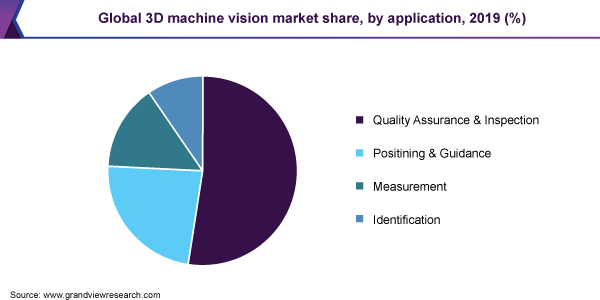
\includegraphics[scale=0.75]{images/3d-vis-market.png}
	}
	\caption{Распределение задач применения систем технического зрения}\label{fig:3d-vis-market}
\end{figure}

Очевидно, что техническое зрение объединяет в себе математические методы, информационные технологии и аппаратную составляющую. Поэтому регламентирующие стандарты описывают широкий спектр применяемых технологий, от установки объективов до каналов передачи данных. К 2009 году количество стандартов достигло критической отметки, и для их координирования и сопоставления между разными рынками технического зрения было инициировано объединение сообществ из Северной Америки (AIA), Европы (EMVA) и Японии (Japan Industrial Imaging Association, JIIA) в так называемую группу ``G3''. На настоящее время существует ряд принятых стандартов, регламентирующих различные моменты проектирования и испытаний СТЗ.

Основным стандартом, регламентирующим применяемые технологии и методы измерений, является EMVA 1288, разработанный Европейской ассоциацией машинного зрения. Он, в основном, сфокусирован на камерах. Целью данного стандарта уже более 15 лет является универсализация характеристик аппаратной части СТЗ и методики испытаний их работы; он позволяет упростить измерения, связанные с качеством изображения, чувствительности сенсора камеры, энергопотреблением СТЗ и другими характеристиками. В основе лежат стандартизированные отчёты EMVA 1288, содержащие базовые значения параметров камеры с приведёнными графиками и таблицами, значительно упрощающие сравнительный анализ применяемых аппаратных средств.

Перечень стандартов от JIIA 2008 года описывает объективы и способы их крепления на корпусах камер. Здесь регламентируются основные размеры применяемых сенсоров, варианты креплений. Чаще всего размеры сенсоров выражаются в долях дюйма, причём не классического, а равного 16 мм. 

Существуют и общепринятые с 90-х годов стандарты подключения камер и протоколов передачи данных. Например, \textbf{Camera Link} --- протокол для работы с интерфейсом видеокамер, созданный на базе National Semiconductor Channel Link. Он описывает передачу данных между видеокамерами и приложениями с высокой скоростью. Существует три конфигурации интерфейса Camera Link, в зависимости от количества чипов сериализации: Base (один чип), Medium (два чипа) и Full (три чипа), соответственно, меняется скорость передачи данных, от 2 до 5,5 Гбит/сек и различается количество пинов в разъеме (рис. \cref{fig:full-cameralink}). В интерфейсе используются сигналы синхронизации видео, управления камерой, связи и питания. Однако, данный стандарт ограничивает длину кабеля 10 метрами, требует дорогостоящего оборудования и не позволяет одновременное использование нескольких камер.

\begin{figure}[ht]
	\centerfloat{
		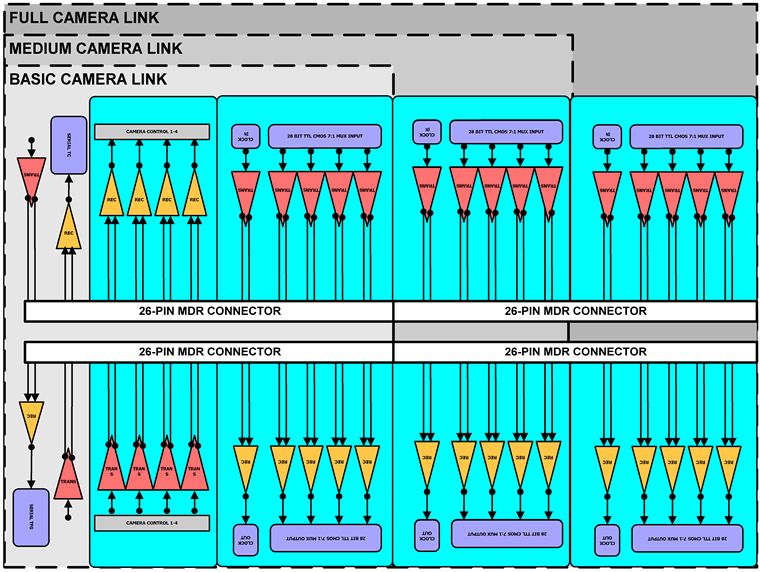
\includegraphics[scale=0.75]{images/full-cameralink.png}
	}
	\caption{Структура интерфейса Camera Link в различных конфигурациях}\label{fig:full-cameralink}
\end{figure}

В качестве преемника Camera Link той же JIIA в 2011 году был представлен \textbf{CoaXPress}, обеспечивающий высокоскоростную передачу данных посредством коаксиального кабеля. Стандарт поддерживает скорость передачи видеопотока до 12,5 Гбит/сек, но с ростом скорости снижается максимальная длина проводного соединения. Однако, CoaXPress пока что не является стандартным для оборудования и требует наличия съемной платы, которая дополнительно будет снижать нагрузку на центральный процессор компьютера.

Также относительно недавно, в 2006 году, Европейской ассоциацией машинного зрения (EMVA) был разработан стак протоколов \textbf{GenICam}, предоставляющий пользователю единый универсальный интерфейс подключения камер различных типов и архитектур. В СТЗ, поддерживающих GenICam, интерфейсы передачи данных обладают взаимозаменяемостью, это же относится и к программному обеспечению систем. Стандарт подразделяется на несколько модулей, каждый из которых выполняет свои функции. Так, GenApi необходим для удалённого конфигурирования параметров камер и управления видеосигналом, а GenTL служит связующим звеном между устройствами и осуществляют передачу данных от камеры к контроллеру с программным обеспечением. Двух вышеуказанных модулей вполне хватает для полноценного функционирования СТЗ.

Кроме вышеперечисленных, существует ещё ряд интерфейсов передачи данных, в том числе проприетарных, характерных для узкоспециализированного оборудования. Однако, для большинства задач достаточно характеристик, имеющихся у \textbf{USB 3.0}. Данный интефейс является развитием USB 2.0 и обеспечивает передачу информации до 5 Гбит/сек и электроэнергии до 900 мА.

\section{Текущее положение систем технического зрения в промышленности} \label{sect1_2}

Промышленность --- одна из немногих отраслей человеческой деятельности, которая вынуждена быть на передовой технологического прогресса. В современном мире уровень потребления товаров населением высок и лишь растёт, кроме того, повышаются требования к качеству и надежности изделий. Повышение скорости производства сказывается на цене для конечного пользователя, а, значит, делает его более привлекательным на рынке, но, вместе с тем, повышается риск падения качества и появления большой доли брака в партии. Сейчас СТЗ занимают важное место в производстве даже самых дешёвых изделий и предоставляют множество функций по автоматизации отдельных операций, выполняемых на оборудовании, например, задачи сборки, сортировки и контроля. Перечень же задач, решаемых СТЗ на производстве, очень широк, сюда входят и дефектоскопия, и отслеживание перемещения заготовки, и контроль фракций и смесей на инородные включения, и контроль сборки узлов и многое другое. Интеграция СТЗ в единую систему, входящую в информационную систему предприятия, позволяет оперировать данными о производстве изделия, агрегировать их, анализировать и совершенствовать техпроцессы. Как известно, большая доля автоматизированного труда является одним из признаков развитой экономики, тогда как в менее развитых странах предпочитают использовать ручной труд.

Другой огромный пласт применения СТЗ в промышленности - это безопасность. Чем сложнее производство, тем более жёсткие требования по технике безопасности оно имеет. Любой несчастный случай на предприятии способен привести к гибели персонала, потере средств на страховые выплаты и к простою оборудования, поэтому имеет смысл вкладываться в автоматизированные решения, снижающие риск появления таких случаев. СТЗ хорошо зарекомендовали себя в задачах промышленной безопасности, например, СТЗ может применяться в задачах отслеживания ношения защитных касок персоналом предприятия или отслеживании появления лиц в запретных для нахождения зонах. К сожалению, не все управляющие кадры решаются внедрять подобные системы, поскольку они обычно очень дороги в установке и в обслуживании, но многие не только западные, но и российские предприятия начинают ставить жизнь работников выше прибылей.

Зачастую СТЗ не являются частью оборудования производственной линии, а действуют обособленно, этакой надстройкой над основной системой управления без обратной связи. Они отправляют ряд сигналов управляющей системе, однако, почти ничего не принимают, продолжая действовать по своим алгоритмам. Иногда большего и не требуется, например, в задачах дефектоскопии, но в условиях изменения производства такие системы нуждаются в перекалибровке и перенастройке, что выливается в дополнительные затраты. В качестве примера такой системы можно рассмотреть СТЗ для определения дефектов прокатного листа, обобщенную структуру которого можно видеть на \cref{fig:cv-line}. Как видно, в упрощенном виде она состоит из одной или нескольких камер, сервера обработки данных и консоли оператора. В случае больших массивов данных можно выделить отдельный контроллер по обработке полученных данных, прежде чем подавать их на ПО СТЗ. Также при необходимости можно внедрить вспомогательные механизмы СТЗ, например, источник освещения или пылесосы, которые будут снижать количество частиц в воздухе. Но самое главное, что видно из этого изображения -- это то, что связь системы с общим дата-центром предприятия сугубо однонаправленная.

\begin{figure}[ht]
	\centerfloat{
		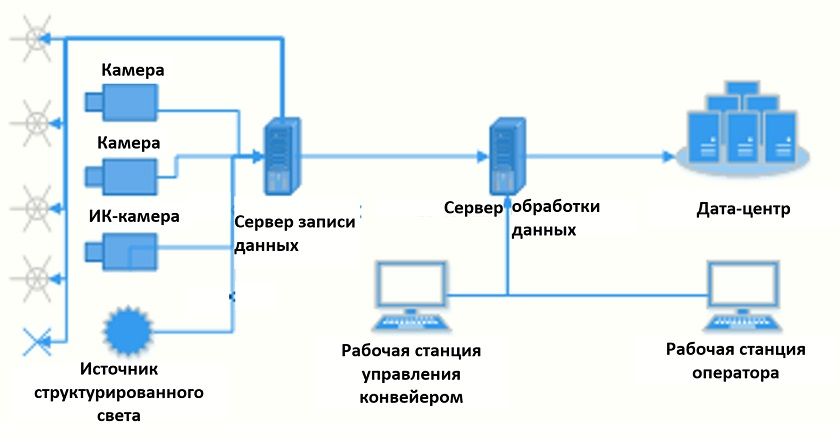
\includegraphics[scale=0.75]{images/cv-line.jpg}
	}
	\caption{Пример структуры СТЗ для контроля качества прокатного листа}\label{fig:cv-line}
\end{figure}

Разумеется, не все системы могут функционировать без обратной связи, в некоторых решениях удалённое конфигурирование необходимо, например, в задачах контроля площадей предприятия под открытым небом. В меняющихся временах суток и погодных условиях важно подстраивать камеру под текущие условия, чтобы СТЗ могла успешно выполнять свои функции.

Чаще всего СТЗ проектируются под требования заказчика ``на месте'', поскольку при развёртывании такой системы требуется учесть множество факторов: расположение камер, уровень освещённости и чистоты воздуха, вибрации и наличие высоких температур. Однако, многие производители предлагают специализированное оборудование для быстрой установки СТЗ, как в виде смонтированного в корпусе обрабатывающего компьютера, так и в виде полноценных комплектов, со своими камерами и другой периферией. Такие системы предлагаются, например, фирмами Delta Electronics, Axiomtek или AAEON. Компьютеры снабжены рядом распространённых разъемов для подключения периферии (рис. \cref{fig:cv-line}) и снабжены собственным ПО для разработки алгоритмов. Такие продукты можно назвать универсальными решениями для производственных нужд. Кроме того, современные технологии позволяют разместить обрабатывающий контроллер в одном корпусе с камерой (например, продукция фирмы Alvium), однако, такие системы сложно назвать подкодящими для высокопроизводительных задач.

\begin{figure}[h]
	\centerfloat{
		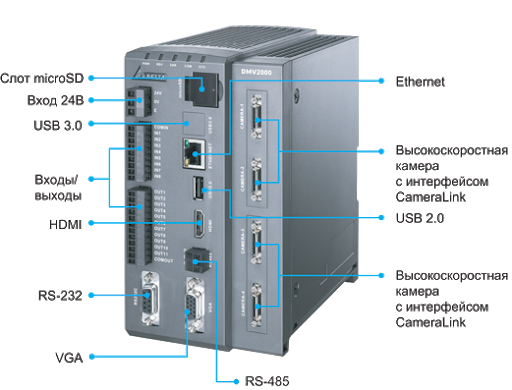
\includegraphics[scale=0.75]{images/delta-el.png}
	}
	\caption{Конфигурация и состав разъёмов на лицевой панели контроллера DMV-2000 от Delta Electronics}\label{fig:delta-el}
\end{figure}

Для конфигурирования подобных систем используется интерфейс оболочки, доступный при подключении периферии или по протоколам удалённого доступа типа VNC или RDP. В качестве языка для составления алгоритмов может использоваться блок-схема, каждый элемент которой выполняет свою функцию с определенными параметрами. Система позволяет выделить интересующий сегмент кадра, настроить параметры изображения с камеры и выбрать интересующую операцию, например, сканирование штрих-кода.

Что касается промышленного оборудования со встроенными СТЗ, то, в основном, речь идёт о сортирующих и сборочных роботах. В случае же обрабатывающего оборудования, например, фрезерных или сверлильных станков, встроенных систем практически не наблюдается. Действительно, обрабатывающее оборудование зачастую составляет лишь малую часть производственной линии и куда проще устанавливать системы инспекции там, где это необходимо. Кроме того, визуальный доступ к зоне обработки изделия чаще всего затруднен самим инструментом и его приводом, паром и воздушными взвесями, а так же защитными экранами и другими возможными помехами.

Таким образом, можно отметить, что СТЗ уже давно стало неотъемлемой частью промышленного производства, сильно поднимающего уровень автоматизации предприятия.Несмотря на то, что часто СТЗ стоят довольно дорого и проектируются под условия заказчика, в перспективе они высвобождают большое количество ресурсов предприятия, сокращают время производства изделия и, соответственно, его стоимость для конечного потребителя.

\section{Уровень разработанности темы в исследованиях} \label{sect1_3}

Подытоживая сказанное в предыдущем разделе, становится очевидным, что научно-технические разработки по данной тематике вызывают интерес не только с научной, но и с практической точки зрения. На текущий момент проблемами использования СТЗ в производственных задачах занимается большое число коллективов из разных стран мира. Поскольку условия на разных производствах сильно разнятся, данная проблематика не теряет актуальности и по сей день, постоянно возникают какие-то уникальные задачи, требующие своего подхода к их решению.

Применение СТЗ в промышленности началось даже до того момента, как они стали более-менее доступными для массового погтребителя. Скажем, штрих-код берёт своё начало аж в 40-х годах прошлого века, а первый раз его отсканировали в 1974 году в супермаркете штата Огайо, США. С тех пор штрих-коды широко применяются в том числе и в задачах идентификации изделия на производственной линии.

В СССР вопросами внедрения технического зрения занимались с 80-х годов прошлого века. При научном Совете АН СССР ``Робототехника и автоматизированное производство'' была сформирована научная группа, занимающаяся системами технического зрения. В неё входили такие авторы, как Титов В.С., Жаботинский Ю.Г., Жданов А.А., Александров Е.И., Якушенков Ю.Г., Соколов С.М., Пряничников В.Е., Ширабакина Т.А., Карели-Лямина Э.С. и другие. В ходе работы были определены концепции построения СТЗ, основные применяемые методы и алгоритмы обработки визуальной информации, классифицированы основые типы СТЗ. Так, среди основных видов СТЗ упоминаются светолокационные, для распознавания символов, для раскроя материала, для контроля распределения температур и т.д. Была приведена обобщенная структура, представленная на рисунке \cref{fig:stz-ussr}, а также обобщенная последовательность действий работы СТЗ.

\begin{figure}[h]
	\centerfloat{
		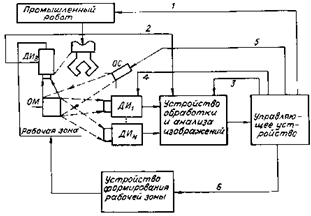
\includegraphics[scale=1.5]{images/stz-ussr.png}
	}
	\caption{Структурная схема СТЗ}\label{fig:stz-ussr}
\end{figure}

Как уже было отмечено ранее, развитие цифровых сенсорных матриц и появление высокоскоростных интерфейсов передачи данных типа USB позволило решать задачи СТЗ в реальном времени и упростило создание таких систем. Внедрение СТЗ в производственные линии существенно упростилось, что подстегнуло создание научных работ по их созданию и внедрению в производство. Стоит отметить, что чаще всего научные работы носят сугубо прикладной характер, решая какую-то узкоспециализированную производственную задачу.

-

\section{Модульный подход в проектировании оборудования с ЧПУ} \label{sect1_4}

Классическая концепция промышленного оборудования предполагает, что станок может выполнять лишь одну или несколько слабо отличающихся друг от друга операций по обработке изделия. Оператор станка может вручную поменять резец или фрезу, варьировать подачу и скорость резания, менять угол режущей кромки, но такие станки остаются не слишком универсальными. Они широко применяются в массовом и крупно серийном производстве и не требуют высокой квалификации от оператора, они дёшевы в производстве и долговечны. Однако, за рамками масового и крупносерийного производтсв применение такого оборудования уже становится неудобным, они могут работать считанные минуты из всей рабочей смены, быстро позволяя выполнять норму обработки и превращаясь в ненужный элемент интерьера в остальное время. Малые производства характеризуются в первую очередь постоянной сменой технологического процесса, поскольку спектр их работы может быть очень широким и вариативным. Грубо говоря, на таких производствах куда больше времени выделяется на подготовку производства, нежели на само производство, а партии товаров редко превышают цифру в несколько тысяч изделий.

Первым шагом к модульности оборудования можно считать сменные инструментальные головки. В ассортименте небольших обрабатывающих станков начали появляться изделия, частично позволяющие конфигурировать инструментальный блок. Чаще всего это станина, на которую навешиваются те или иные элементы, превращая станов в фрезерный, товарный, сверлильный и т.д. Это так называемая ``Механическая модульность'', компоненты связаны друг с другом лишь креплениями, а их установка обычно производится вручную. Данное оборудование можно назвать универсальным, но лишь в рамках производимых им обрабатывающих операций. Такие станки выпускает, к примеру, компания Unimat (рис. \cref{fig:unimat_ml_technics}), оборудование собирается по принципу конструктора из составляющих частей.

\begin{figure}[h]
	\centerfloat{
		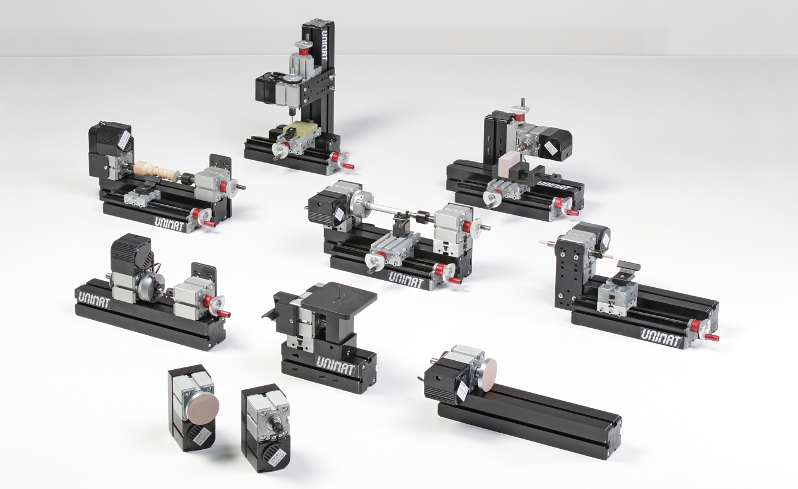
\includegraphics[width=\textwidth]{images/unimat_ml_technics.png}
	}
	\caption{Конструктор станков для механической обработки от компании Unimat}\label{fig:unimat_ml_technics}
\end{figure}

Однако в области модульного подхода можно пойти ещё дальше, реализовав распределенную систему управления и взаимосвязи модулей между собой. Модули могут быть связаны между собой не только физически, но и посредством ЛВС, а то и только посредством ЛВС, при этом находясь на некотором отдалении от базовой платформы. Таким образом можно выстраивать целые производственные линии из разного оборудования. Развитие беспроводных сетей типа Wi-Fi и ZigBee позволяет организовать централизованную или же децентрализованную систему управления, участники которой могут находиться хоть в разных помещениях. Таким образом, можно быстро перестраивать технологические процессы в зависимости от текущего заказа, а уровень автоматизации производства при правильной организации будет очень высоким. Такая концепция оборудования называется ``многоагентной системой''.

Однако, есть вопрос о способе коммуникации модулей в процессе конфигурирования или процесса работы. Существует несколько концепций взаимодействия модулей между собой, первой из которых можно назвать систему, основанную на ``холонах''\footnote{Термин, предложенный Артуром Кестлером для описания биологических систем}. Суть концепции заключается в том, что компоненты системы равны друг другу и могут образовывать устойчивые связи друг с другом в рамках системы, если это необходимо (рис. \cref{fig:holonic-struc}). Иными словами, данная концепция предполагает существование обособленных систем внутри изначальной. Холоническая структура относится к классу гетерархических структур, т.е., структур без ярко выраженного центра. Холоны могут дополнять друг друга внутри конкретной системы, и разделяться на высшие и низшие уровни. Связи, выстраиваемые между холонами (холархии), имеют динамический характер и легко перестраиваются в ответ на воздействие неких внешних сред, а сам холон может быть частью нескольких холархий одновременно. Проблемами холонических систем занимались А. Коломбо, П. Лейтао, Л.~Я. Дорфман, К. Гербер и другие.

\begin{figure}[h]
	\centerfloat{
		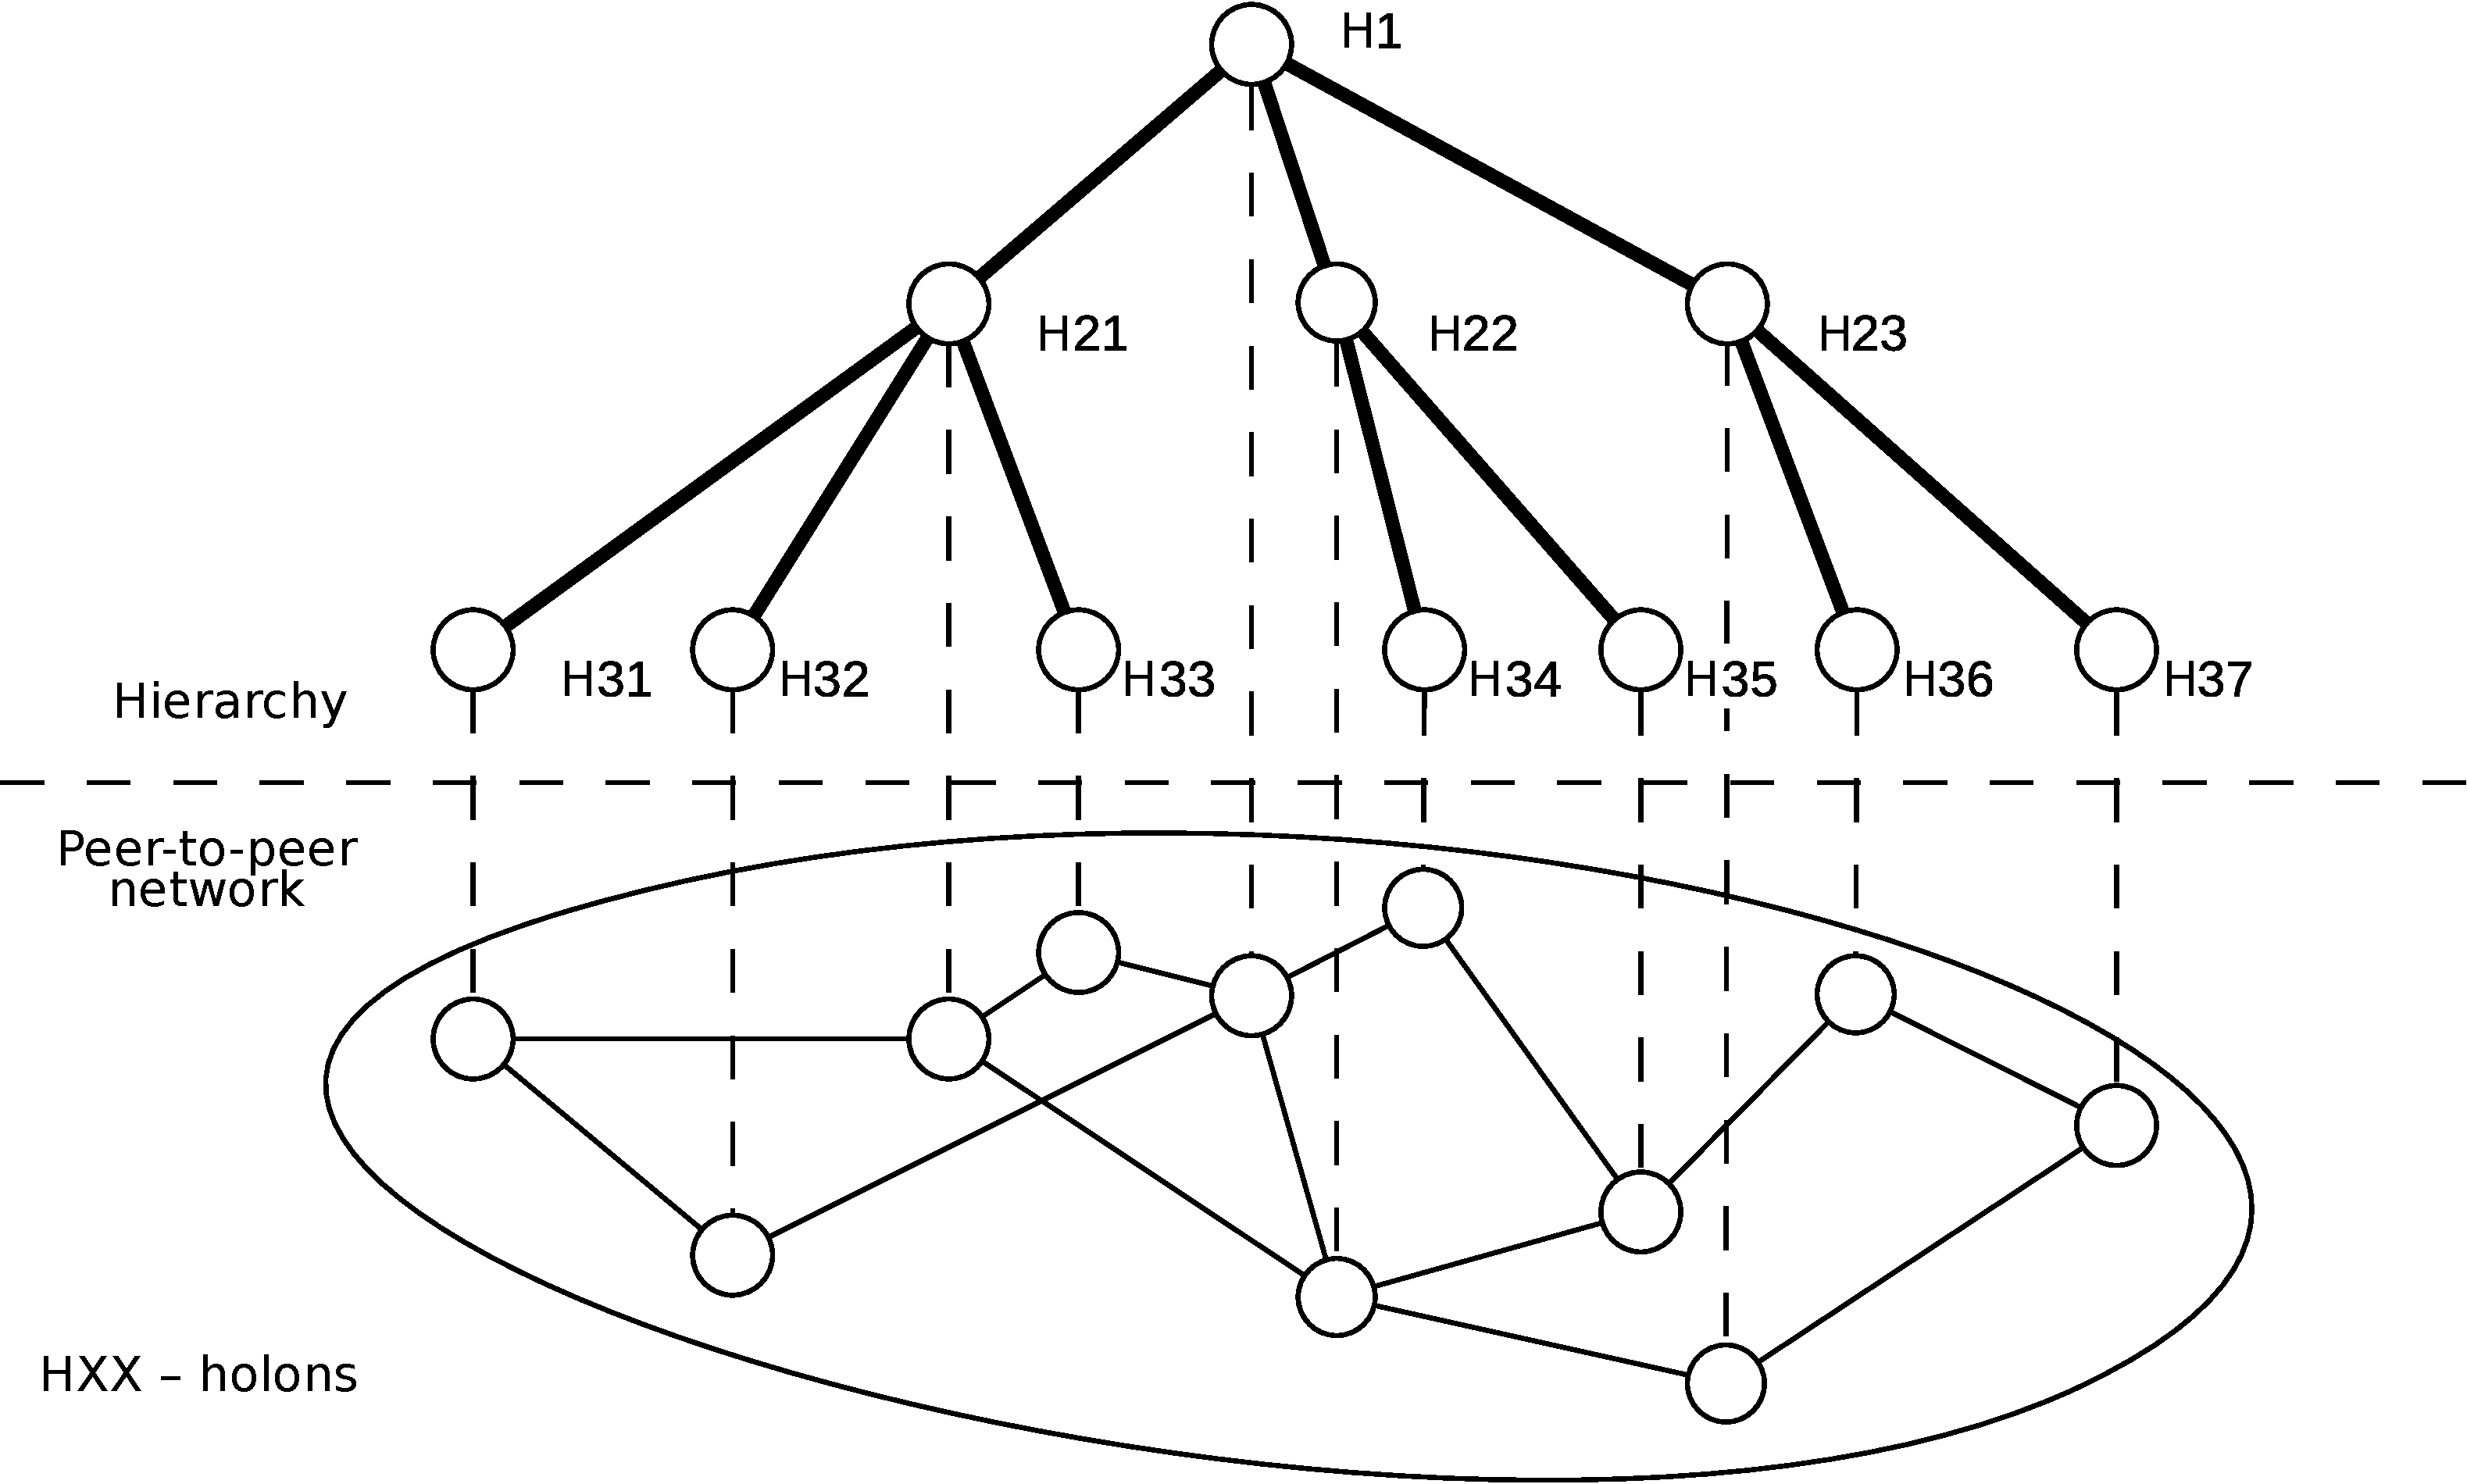
\includegraphics[width=15cm]{images/holonic-struc.pdf}
	}
	\caption{Структура многоуровневой холонической системы}\label{fig:holonic-struc}
\end{figure}

Второй концепцией взаимодействия модулей можно назвать микросервисную архитектуру. Это современная интерпретация так называемых сервис-ориентированных моделей, применяющихся в распределённых программных системах. Микросервисная модель также децентрализована, а под сервисом в ней понимается процесс операционной системы, взаимодействующий с другими процессами для выполнения определённой задачи. Архитектура микросервисов использует общий протокол коммуникации, поэтому модули легко подвергаются замене при необходимости. Сами модули при этом организованы вокруг функций, которую может предоставить тот или иной микросервис, а сами микросервисы сильно ограничены в своих возможностях и могут выполнять только одну функцию. Концепция описывается в работах А. Коломбо, Р. да Силвы, Т. Вреска и других авторов.

\begin{figure}[ht]
	\centerfloat{
		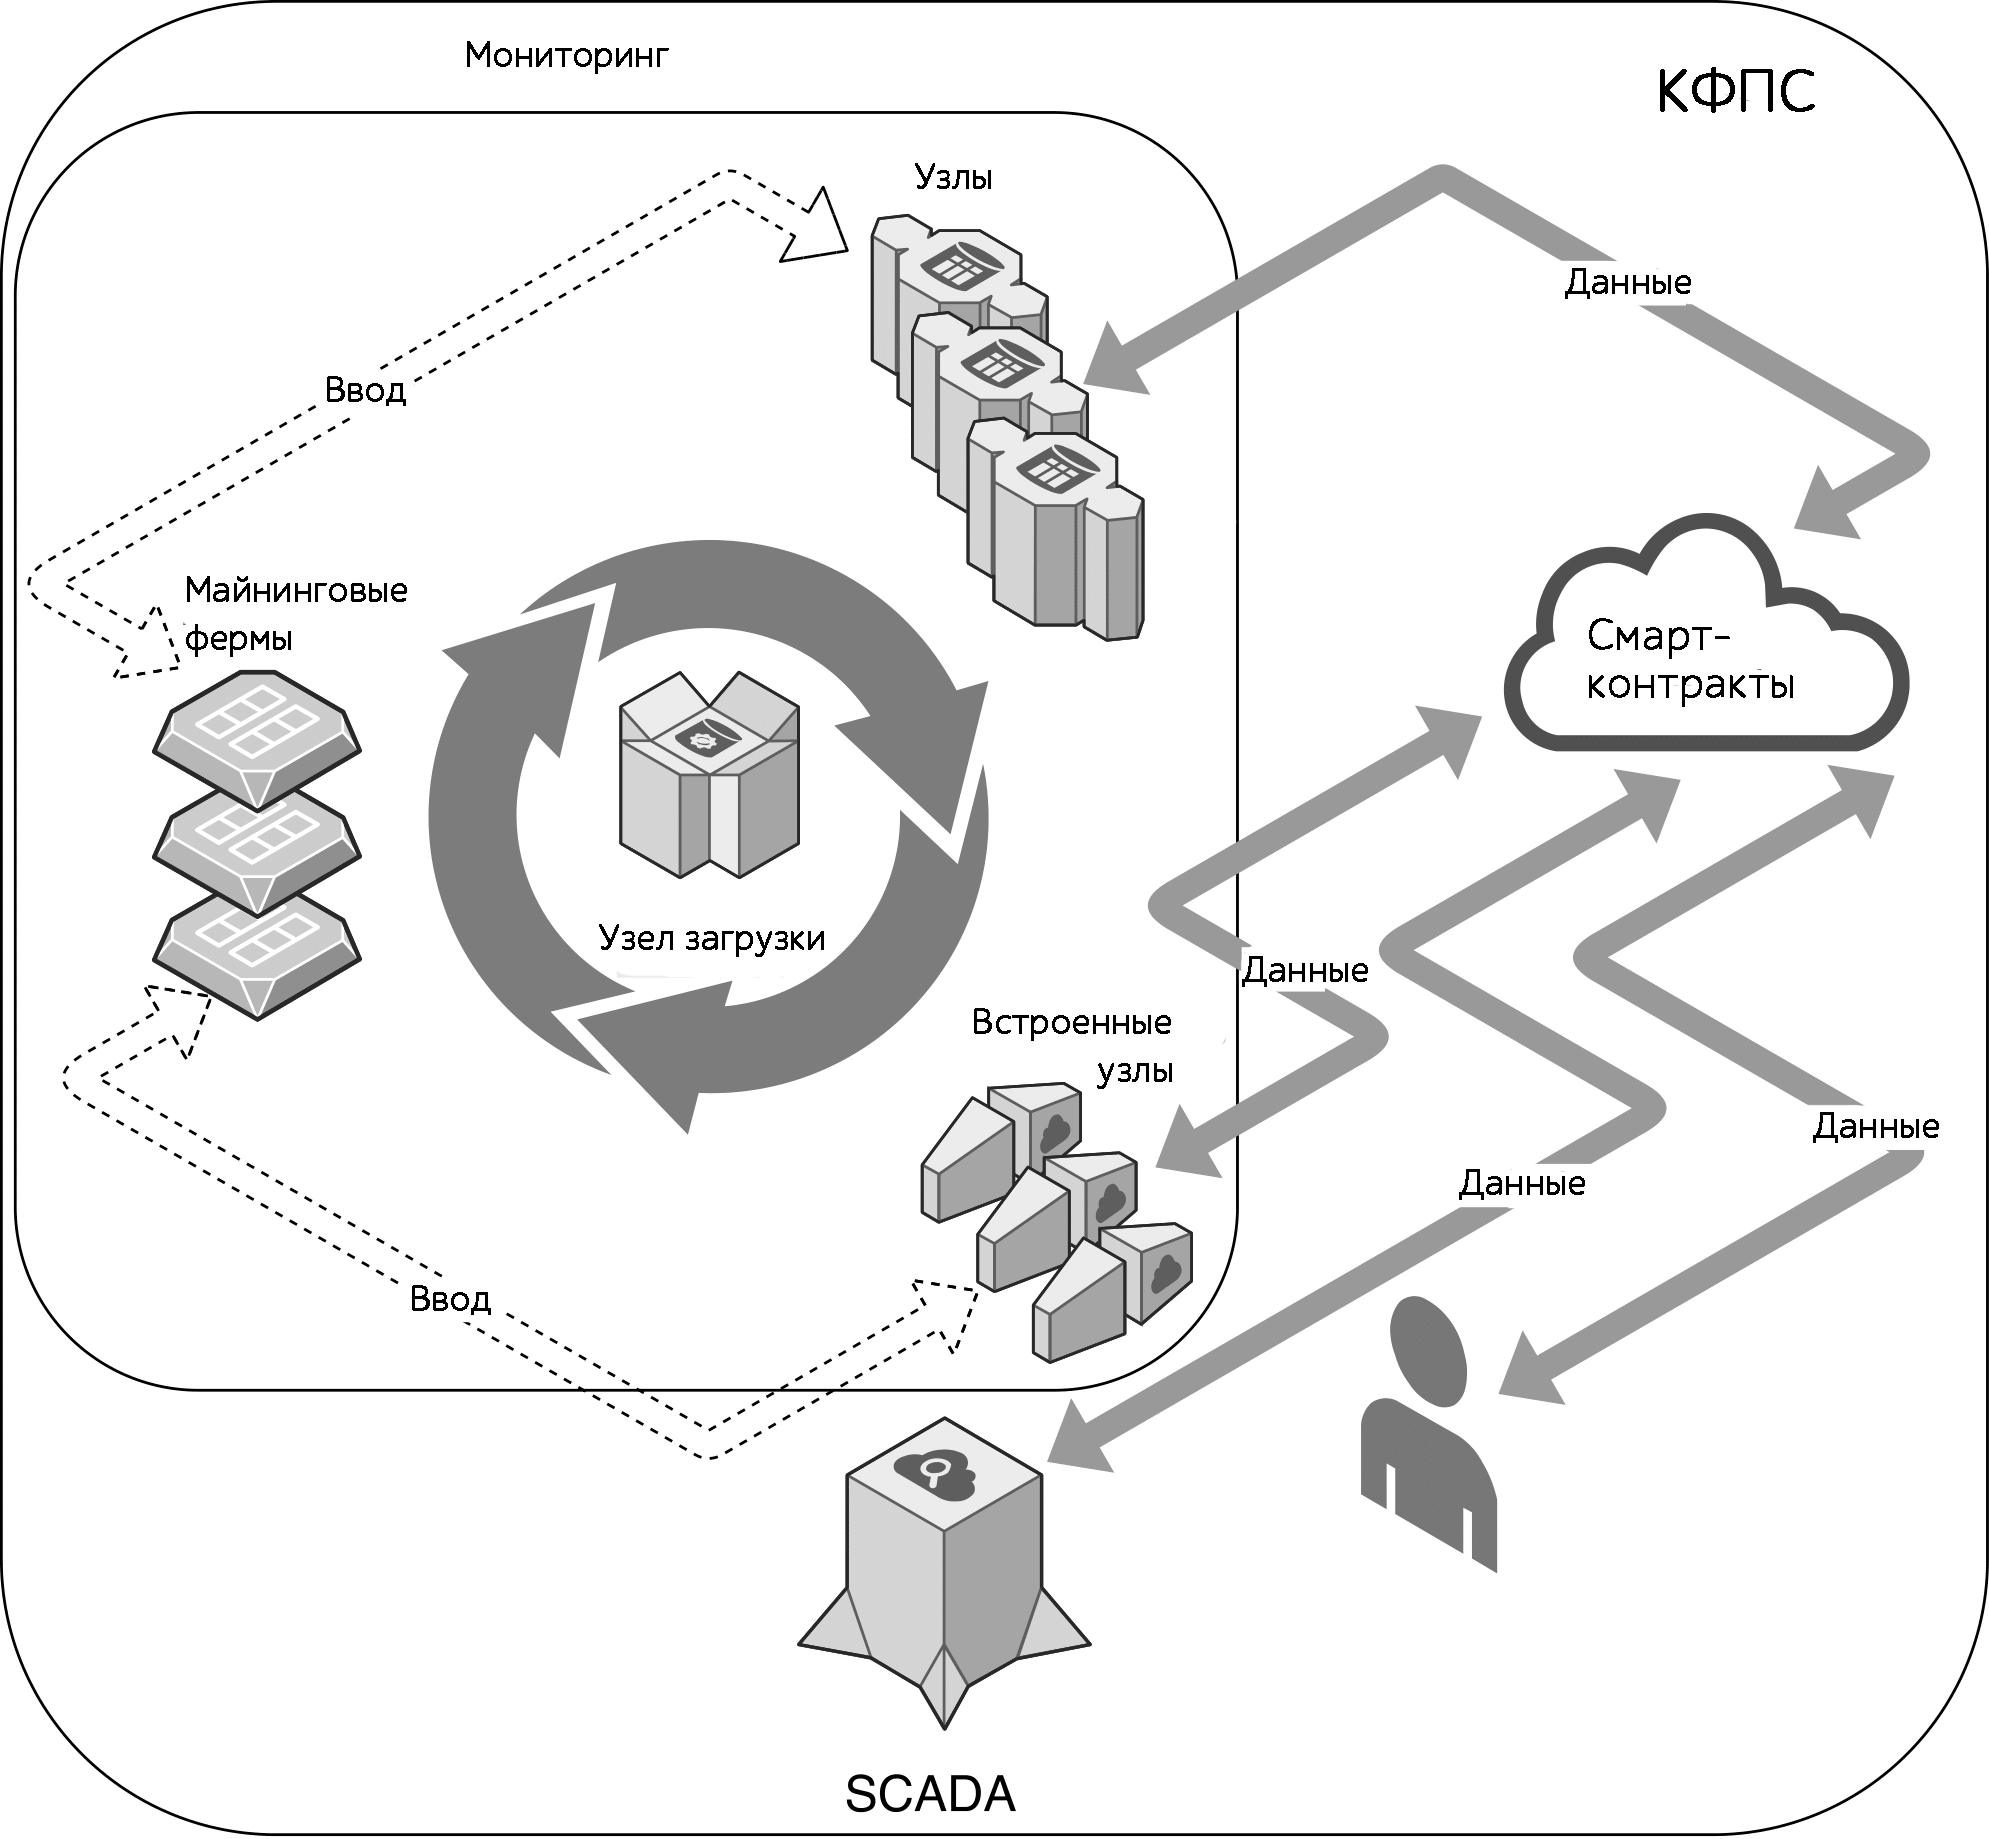
\includegraphics[width=15cm]{images/bc-system.png}
	}
	\caption{Модель блокчейн-ориентированной системы}\label{fig:bc-system}
\end{figure}

Еще одной интересной концепцией межмашинного взаимодействия является применение блокчейна и смарт-контрактов. Смарт-контрактом называется самоисполняющийся сценарий, реализованный на специализиованном языке программирования, что позволяет проводить операции без участия третьих лиц. Создать смарт-контракт может любой участник сети, поэтому данная концепция вполне подходит для организации распределённой системы управления (рис. \cref{fig:bc-system}). Стоит отметить, что для этого лучше использовать частный блокчейн, чья крипто-валюта не привязана к бирже и не имеет стоимости на рынке. При помощи блокчейна обеспечивается не только межмашинное взаимодействие, но и протоколы безопасности, единая информационная среда, а также возможность масштабирования и реструктуризации. Данную концепцию в своих работах описывали Н. Тесля, К. Кристидис и Ф. Биккафурри.

Таким образом, можно сказать, что модульное оборудование развилось до сложных самоорганизующихся систем, которое предоставляет куда больше возможностей, чем классические централизованные системы управления. Помимо перечисленных концепций, существуют ещё другие, к примеру, ``Fog of Things'', что подчеркивает широкий интерес исследователей к теме межмашинного взаимодействия.

\section{Описание разрабатываемой модульной трёхкоординатной платформы} \label{sect1_5}

Разрабатываемая трехкоординатная платформа относится к категории малого модульного оборудования с ЧПУ и предназначена для выполнения техпроцессов изделий широкой номенклатуры. Данное оборудование предполагается к использованию в лабораториях и на малых предприятиях для производства прототипов и малых партий изделий. Ключевой характеристикой платформы является возможность создания на ее базе разные виды высокотехнологичного оборудования для реализации как обрабатывающих, так и вспомогательных операций, что, безусловно, является важным качеством для небольших стартапов, ориентированных на широкое разнообразие выпускаемых изделий.

Основным компонентом трёхкоординатной платформы является, собственно, шасси, оснащенное приводами с шаговыми двигателями, позволяющими каретке перемещаться над рабочей зоной. Рендер модели шасси представлен на рисунке \cref{fig:table-r}. Размер рабочей зоны составляет 500 на 500 мм, онако, предполагается создание и более крупных платформ. На каретку могут устанавливаться модули, выполняющие разную инструментальную обработку: фрезерный, сверлильный, лазерный и т.д. Крепление модулей осуществляется при помощи электромагнитов, установленных с обеих сторон каретки.

\begin{figure}[ht]
	\centerfloat{
		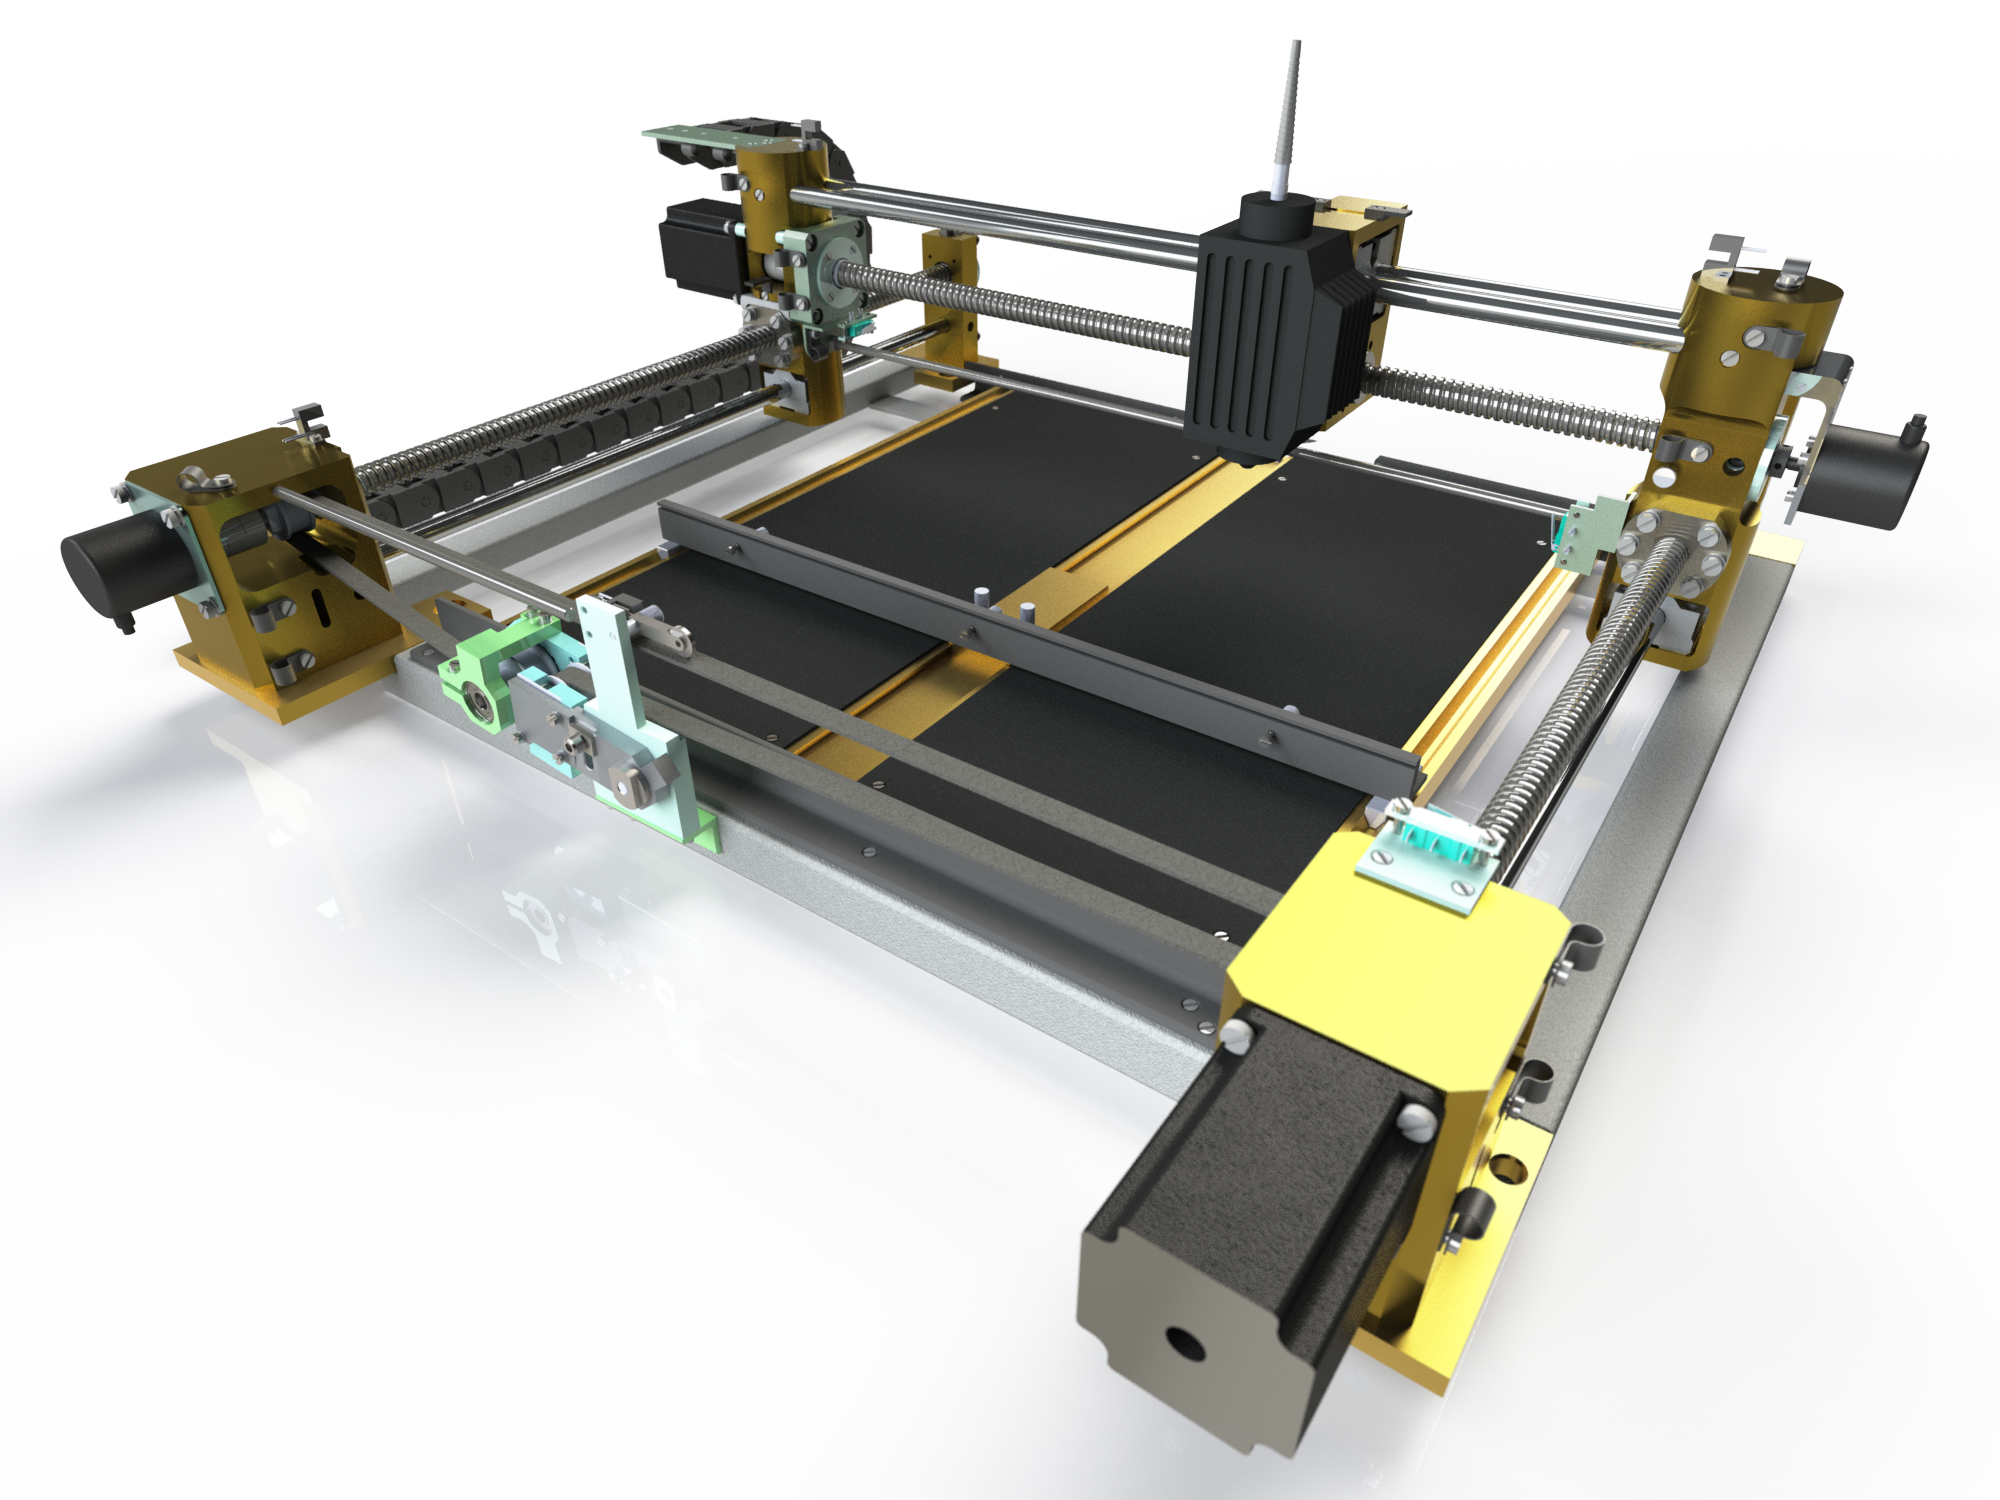
\includegraphics[width=15cm]{images/table-r.png}
	}
	\caption{Внешний вид трехкоординатной платформы (рендер)}\label{fig:table-r}
\end{figure}

Среди вспомогательных операций можно выделить контролирующие, измерительные, калибровочные и транслирующие. Здесь не последнюю роль играет модуль СТЗ, интегрированный в систему управления платформы. При помощи СТЗ выполняется контроль положения и выполнения операций над заготовкой, измерения касаются сборочных и установочных операций, калибровка неоходима для связи системы координат инструмента на модуле с системой координат платформы, а транслировать предполагается ход работ с целью дальшейшего анализа техпроцесса и выявления нештатных ситуаций. Подробнее о функциях и задачах СТЗ платформы будет описано в главе 3 настоящей диссертационной работы.

Взаимосвязь модулей осуществляется посредством беспроводной локальной сети. Каждый модуль имеет свой набор параметров, который он при первом подключении отправляет в сеть и который организован в виде файла JSON со структурой, представленной на рисунке \cref{fig:json}. Данная структура позволяет изменять параметры оборудования при необходимости как вручную, так и управляющей программой. Среди параметров модуля прописывается его физический адрес в сети, разрешённые функции с G-кодами, название и перечень параметров с максимально и минимально допустимыми значениями. Все файлы с параметрами прописываются в реестре каждого модуля. Для коммуникации используется OpenThread, одна из реализаций спецификации IEEE 802.15.4, поскольку он открытый и ориентирован на передачу IPv6-трафика. В качестве топологии применяется ячеистая сеть, позволяющая связать каждый модуль друг с другом на одном уровне.

\begin{figure}[ht]
	\centerfloat{
		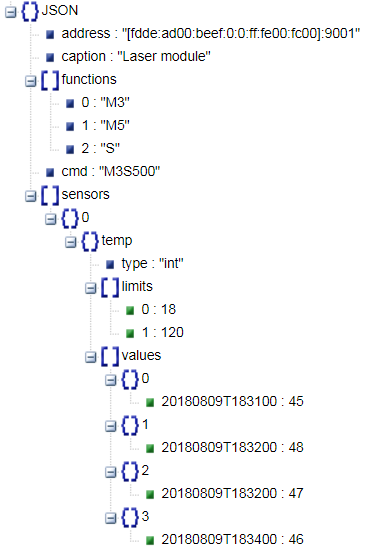
\includegraphics[width=8cm]{images/json.png}
	}
	\caption{Структура параметров модуля, отображенная в передаваемом файле типа JSON}\label{fig:json}
\end{figure}

Важно отметить, что данная платформа в настоящий момент находится в статусе доработки, поэтому многие моменты ещё не протестированы должным образом. Однако, общая концепция оборудования уже определена и является основным референсом в доработках и отладках.

\section{Выводы по первой главе} \label{sect1_6}

В данной главе были упомянуты общие положения систем визуального анализа, области их применения и существующие стандарты. В текущем разнообразии технических средств, развитии информационных технологий и появления фреймворков для создания СТЗ важно сохранять единство параметров, протоколов и каналов передачи данных. Стандарты касаются не только аппаратной, но и программной составляющих СТЗ.

Применение СТЗ в промышленности также является широко обсуждаемой темой. Всё больше предприятий в России и за рубежом повсеместно внедряют СТЗ для выполнения самых разных задач: дефектоскопия, отслеживание, техника безопасности и т.д.

Был рассмотрен богатый научный бэкграунд, сформированный за долгие десятилетия работы с СТЗ в разных сферах деятельности. Развитие СТЗ в области промышленного производства берёт своё начало из 70-х и 80-х годов, когда методы ещё только нарабатывались, а компьютеры были недоступны большинству заинтересованных лиц. Но, постепенно, с развитием транзисторной электроники и высокосоростных каналов передачи данных количество работ начало расти, а создание простой СТЗ уже не вызывает трудностей.

Также была описана разрабатываемая трехкоординатная платформа, представлена её структура и технические характеристики. Платформа относится к модульному оборудованию с ЧПУ и предназначена для производства изделий широкой номенклатуры. Данное оборудование является базой в исследованиях, посвященных созданию и ипользованию СТЗ в промышленных станках.